\chapter{HASIL PENELITIAN DAN PEMBAHASAN}
Bab ini terdiri atas tiga bagian, yakni hasil penelitian, pembahasan, dan keterbatasan penelitian. Subbab pada bab 4 ini dapat disesuaikan dengan kebutuhan. Uraikan bab ini sesuai dengan alur berpikir dalam diagram alir

\section{Hasil Penelitian}
Hasil penelitian harus menjawab pertanyaan penelitian dan disusun menurut urutan pertanyaan penelitian/hipotesis.

\subsection{Pengelompokan Jenis Roti}
\begin{longtable}{|l|l|l|}
	\caption{Pengelompokan jenis roti di Lyly Bakery Lamongan} \\
	\hline
	No & Pengelompokan & Jenis Roti \\ \hline
	\multirow{10}{*}{1} & \multirow{10}{*}{Donat} & Donat strawberry marble \\ \cline{3-3}
	& & Donat chocolate peanut \\ \cline{3-3}
	& & Donat chocolate marble \\ \cline{3-3}
	& & Donat white choco almond \\ \cline{3-3}
	& & Donat icing sugar \\ \cline{3-3}
	& & Donat misis mix \\ \cline{3-3}
	& & Donat misis coklat \\ \cline{3-3}
	& & Donat chicken \\ \cline{3-3}
	& & Donat keju \\ \cline{3-3}
	& & Donat merah putih \\ \hline
	\multirow{7}{*}{2} & \multirow{7}{*}{Pastry Croissant} & Cum-cum contong mini \\ \cline{3-3}
	& & Cum cum sepatu \\ \cline{3-3}
	& & Croissant coklat marble \\ \cline{3-3}
	& & Croissant white almond \\ \cline{3-3}
	& & Grem kacang \\ \cline{3-3}
	& & Fruit danish \\ \cline{3-3}
	& & Apple danish \\ \hline
	\multirow{2}{*}{3} & \multirow{2}{*}{Puff pastry} & Molen coklat \\ \cline{3-3}
	& & Molen keju \\ \hline
	\multirow{6}{*}{4} & \multirow{6}{*}{Tawar} & Tawar kombinasi \\ \cline{3-3}
	& & Tawar kotak \\ \cline{3-3}
	& & Tawar kupas \\ \cline{3-3}
	& & Tawar kupas pandan \\ \cline{3-3}
	& & Tawar zebra \\ \cline{3-3}
	& & Tawar panjang roppang \\ \hline
	\multirow{2}{*}{5} & \multirow{2}{*}{Ban} & Ban hongkong \\ \cline{3-3}
	& & Ban hongkong pandan \\ \hline
	\multirow{8}{*}{6} & \multirow{8}{*}{Cupcake} & Cupcake fondan panda cewek \\ \cline{3-3}
	& & Cupcake fondan panda cowok \\ \cline{3-3}
	& & Cupcake white purple flower \\ \cline{3-3}
	& & Cupcake oreo choco cream \\ \cline{3-3}
	& & Cupcake cactus \\ \cline{3-3}
	& & Cupcake sesame street blue \\ \cline{3-3}
	& & Cupcake sesame street yellow \\ \cline{3-3}
	& & Cupcake kumbang \\ \hline
\end{longtable}

\subsection{Indeks Sensitivitas}
\begin{figure}[h!]
	\centering
	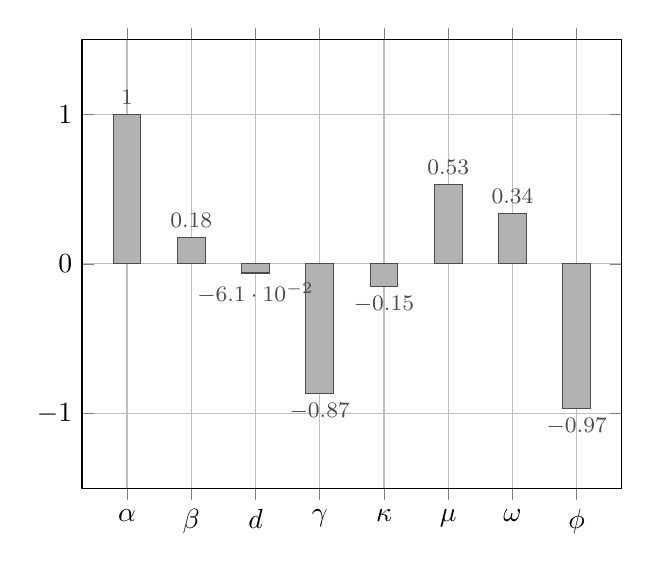
\begin{tikzpicture}
		\begin{axis}[
			ybar,
			ymin=-1.5,
			ymax=1.5,
			symbolic x coords={$\alpha$,$\beta$,$d$,$\gamma$,$\kappa$,$\mu$,$\omega$,$\phi$},
			xtick=data,
			nodes near coords,
			nodes near coords align={vertical},
			nodes near coords style={font=\footnotesize},
			grid=major,
			]
			\addplot[
			color=black!70,
			fill=black!30,
			] coordinates {
				($\alpha$,1)
				($\beta$,0.175)
				($d$,-0.061)
				($\gamma$,-0.87)
				($\kappa$, -0.15)
				($\mu$, 0.53)
				($\omega$, 0.34)
				($\phi$, -0.97)
			};
		\end{axis}
	\end{tikzpicture}
	\caption{Indeks sensitivitas}
\end{figure}

\subsection{Graf}
\begin{figure}[h!]
	\centering
	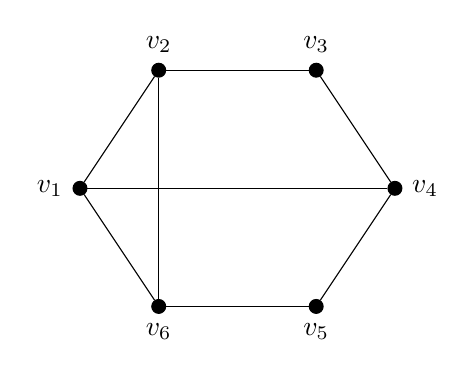
\begin{tikzpicture}[scale=1]
		% Nodes
		\node[circle, draw, fill=black, minimum size=5pt, inner sep=0pt, label=left:$v_1$] (v1) at (0,0) {};
		\node[circle, draw, fill=black, minimum size=5pt, inner sep=0pt, label=above:$v_2$] (v2) at (1,1.5) {};
		\node[circle, draw, fill=black, minimum size=5pt, inner sep=0pt, label=above:$v_3$] (v3) at (3,1.5) {};
		\node[circle, draw, fill=black, minimum size=5pt, inner sep=0pt, label=right:$v_4$] (v4) at (4,0) {};
		\node[circle, draw, fill=black, minimum size=5pt, inner sep=0pt, label=below:$v_5$] (v5) at (3,-1.5) {};
		\node[circle, draw, fill=black, minimum size=5pt, inner sep=0pt, label=below:$v_6$] (v6) at (1,-1.5) {};
		
		% Edges
		\draw (v1) -- (v2);
		\draw (v1) -- (v6);
		\draw (v1) -- (v4);
		\draw (v2) -- (v3);
		\draw (v3) -- (v4);
		\draw (v4) -- (v5);
		\draw (v5) -- (v6);
		\draw (v6) -- (v2);
		\draw (v6) -- (v5);
		\draw (v2) -- (v3);
	\end{tikzpicture}
	\caption{Graf $G$}
\end{figure}

\begin{figure}[h!]
	\centering
	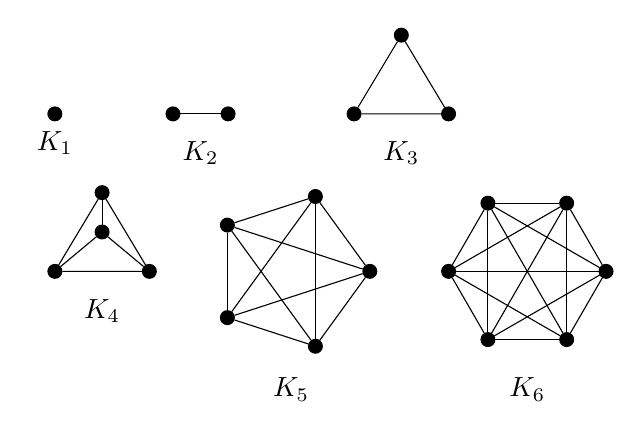
\begin{tikzpicture}[scale=1]
		
		% Row 1: K1, K2, K3
		% K1
		\node[circle, draw, fill=black, minimum size=5pt, inner sep=0pt, label=below:$K_1$] (k1) at (0,1) {};
		
		% K2
		\node[circle, draw, fill=black, minimum size=5pt, inner sep=0pt] (k21) at (1.5,1) {};
		\node[circle, draw, fill=black, minimum size=5pt, inner sep=0pt] (k22) at (2.2,1) {};
		\draw (k21) -- (k22);
		\node at (1.85,0.5) {$K_2$};
		
		% K3 (Triangle)
		\node[circle, draw, fill=black, minimum size=5pt, inner sep=0pt] (k31) at (3.8,1) {};
		\node[circle, draw, fill=black, minimum size=5pt, inner sep=0pt] (k32) at (5,1) {};
		\node[circle, draw, fill=black, minimum size=5pt, inner sep=0pt] (k33) at (4.4,2) {};
		\draw (k31) -- (k32) -- (k33) -- (k31);
		\node at (4.4,0.5) {$K_3$};
		
		% Row 2: K4, K5, K6
		% K4 (Tetrahedron)
		\node[circle, draw, fill=black, minimum size=5pt, inner sep=0pt] (k41) at (0,-1) {};
		\node[circle, draw, fill=black, minimum size=5pt, inner sep=0pt] (k42) at (1.2,-1) {};
		\node[circle, draw, fill=black, minimum size=5pt, inner sep=0pt] (k43) at (0.6,0) {};
		\node[circle, draw, fill=black, minimum size=5pt, inner sep=0pt] (k44) at (0.6,-0.5) {};
		\draw (k41) -- (k42) -- (k43) -- (k41);
		\draw (k41) -- (k44) -- (k42);
		\draw (k43) -- (k44);
		\node at (0.6,-1.5) {$K_4$};
		
		% K5 (Pentagon)
		\foreach \i in {0,72,144,216,288} {
			\node[circle, draw, fill=black, minimum size=5pt, inner sep=0pt] (k5\i) at ({3 + cos(\i)}, {-1 + sin(\i)}) {};
		}
		\foreach \i in {0,72,144,216,288} {
			\foreach \j in {0,72,144,216,288} {
				\ifnum\i<\j
				\draw (k5\i) -- (k5\j);
				\fi
			}
		}
		\node at (3,-2.5) {$K_5$};
		
		% K6 (Hexagon)
		\foreach \i in {0,60,120,180,240,300} {
			\node[circle, draw, fill=black, minimum size=5pt, inner sep=0pt] (k6\i) at ({6 + cos(\i)}, {-1 + sin(\i)}) {};
		}
		\foreach \i in {0,60,120,180,240,300} {
			\foreach \j in {0,60,120,180,240,300} {
				\ifnum\i<\j
				\draw (k6\i) -- (k6\j);
				\fi
			}
		}
		\node at (6,-2.5) {$K_6$};
		
	\end{tikzpicture}
	\caption{Graf Komplit}
\end{figure}

\begin{figure}[h!]
	\centering
	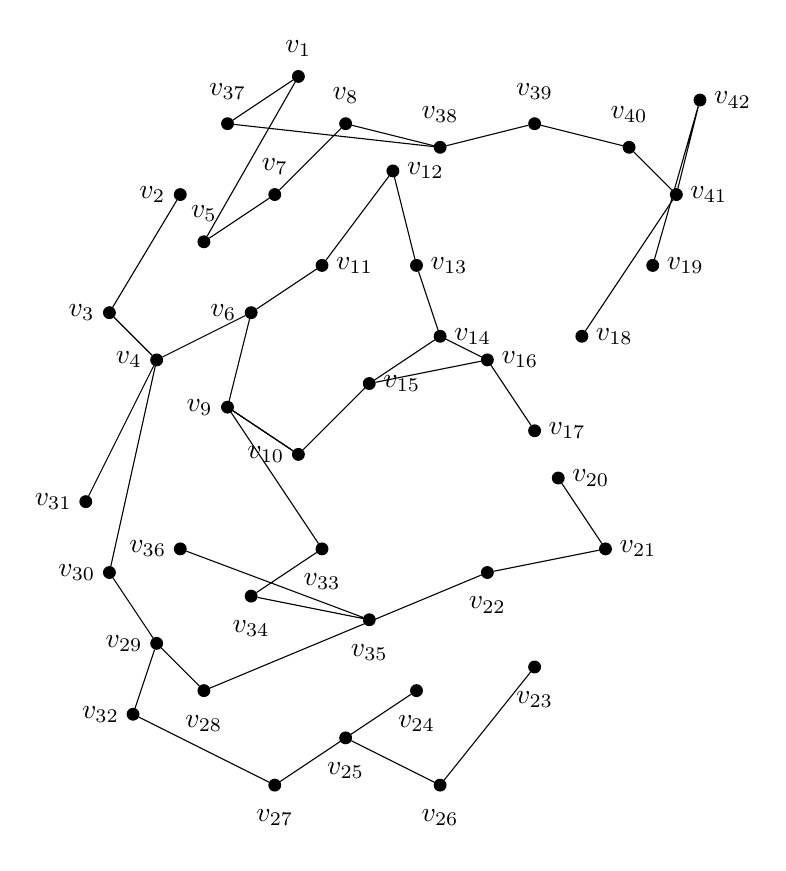
\begin{tikzpicture}[scale=3, every node/.style={circle, draw, fill=black, inner sep=1.5pt}]
		% Penempatan simpul berdasarkan estimasi dari gambar
		\node (v1) at (0,2) [label=above:$v_1$] {};
		\node (v2) at (-0.5,1.5) [label=left:$v_2$] {};
		\node (v3) at (-0.8,1) [label=left:$v_3$] {};
		\node (v4) at (-0.6,0.8) [label=left:$v_4$] {};
		\node (v5) at (-0.4,1.3) [label=above:$v_5$] {};
		\node (v6) at (-0.2,1) [label=left:$v_6$] {};
		\node (v7) at (-0.1,1.5) [label=above:$v_7$] {};
		\node (v8) at (0.2,1.8) [label=above:$v_8$] {};
		\node (v9) at (-0.3,0.6) [label=left:$v_9$] {};
		\node (v10) at (0,0.4) [label=left:$v_{10}$] {};
		\node (v11) at (0.1,1.2) [label=right:$v_{11}$] {};
		\node (v12) at (0.4,1.6) [label=right:$v_{12}$] {};
		\node (v13) at (0.5,1.2) [label=right:$v_{13}$] {};
		\node (v14) at (0.6,0.9) [label=right:$v_{14}$] {};
		\node (v15) at (0.3,0.7) [label=right:$v_{15}$] {};
		\node (v16) at (0.8,0.8) [label=right:$v_{16}$] {};
		\node (v17) at (1,0.5) [label=right:$v_{17}$] {};
		\node (v18) at (1.2,0.9) [label=right:$v_{18}$] {};
		\node (v19) at (1.5,1.2) [label=right:$v_{19}$] {};
		\node (v20) at (1.1,0.3) [label=right:$v_{20}$] {};
		\node (v21) at (1.3,0) [label=right:$v_{21}$] {};
		\node (v22) at (0.8,-0.1) [label=below:$v_{22}$] {};
		\node (v23) at (1,-0.5) [label=below:$v_{23}$] {};
		\node (v24) at (0.5,-0.6) [label=below:$v_{24}$] {};
		\node (v25) at (0.2,-0.8) [label=below:$v_{25}$] {};
		\node (v26) at (0.6,-1) [label=below:$v_{26}$] {};
		\node (v27) at (-0.1,-1) [label=below:$v_{27}$] {};
		\node (v28) at (-0.4,-0.6) [label=below:$v_{28}$] {};
		\node (v29) at (-0.6,-0.4) [label=left:$v_{29}$] {};
		\node (v30) at (-0.8,-0.1) [label=left:$v_{30}$] {};
		\node (v31) at (-0.9,0.2) [label=left:$v_{31}$] {};
		\node (v32) at (-0.7,-0.7) [label=left:$v_{32}$] {};
		\node (v33) at (0.1,0) [label=below:$v_{33}$] {};
		\node (v34) at (-0.2,-0.2) [label=below:$v_{34}$] {};
		\node (v35) at (0.3,-0.3) [label=below:$v_{35}$] {};
		\node (v36) at (-0.5,0) [label=left:$v_{36}$] {};
		\node (v37) at (-0.3,1.8) [label=above:$v_{37}$] {};
		\node (v38) at (0.6,1.7) [label=above:$v_{38}$] {};
		\node (v39) at (1,1.8) [label=above:$v_{39}$] {};
		\node (v40) at (1.4,1.7) [label=above:$v_{40}$] {};
		\node (v41) at (1.6,1.5) [label=right:$v_{41}$] {};
		\node (v42) at (1.7,1.9) [label=right:$v_{42}$] {};
		
		% Koneksi antar simpul sesuai gambar
		\draw (v1) -- (v37) -- (v38) -- (v39) -- (v40) -- (v41) -- (v42) -- (v19);
		\draw (v1) -- (v5) -- (v7) -- (v8) -- (v38);
		\draw (v2) -- (v3) -- (v4) -- (v6) -- (v9) -- (v10);
		\draw (v6) -- (v11) -- (v12) -- (v13) -- (v14) -- (v16) -- (v17);
		\draw (v9) -- (v33) -- (v34) -- (v35) -- (v36);
		\draw (v31) -- (v4) -- (v30) -- (v29) -- (v28);
		\draw (v29) -- (v32) -- (v27) -- (v24) -- (v25) -- (v26) -- (v23);
		\draw (v20) -- (v21) -- (v22);
		\draw (v18) -- (v41);
		\draw (v22) -- (v28);
		\draw (v14) -- (v15);
		\draw (v9) -- (v10) -- (v15) -- (v16);
		
	\end{tikzpicture}
	\caption{Graf Dual}
	\label{fig:Dual}
\end{figure}
Berdasarkan~\ref{fig:Dual}, graf tersebut dapat direpresentasikan dalam titik dan sisi sebagai berikut:
\begin{align*}
	G &= (V(G), E(G))\\
	V &= \left\lbrace 
	\begin{array}{llllllll}
		v_1, & v_2, & v_3, & v_4, & v_5, & v_6, & v_7, & v_8,\\
		v_9, & v_{10}, & v_{11}, & v_{12}, & v_{13}, & v_{14}, & v_{15}, & v_{16},\\
		v_{17}, & v_{18}, & v_{19}, & v_{20}, & v_{21}, & v_{22}, & v_{23}, & v_{24},\\
		v_{25}, & v_{26}, & v_{27}, & v_{28}, & v_{29}, & v_{30}, & v_{31}, & v_{32},\\
		v_{33}, & v_{34}, & v_{35}, & v_{36}, & v_{37}, & v_{38}, & v_{39}, & v_{40},\\
		v_{41}, & v_{42}
	\end{array}
	\right\rbrace
\end{align*}

\begin{align*}
	E &= \left\lbrace 
	\begin{array}{llllllll}
		(v_1v_2), & (v_1v_{37}), & (v_2v_3), & (v_2v_4), & (v_2v_5), & (v_2v_{37}), & (v_3v_4), & (v_3v_{30}),\\
		(v_4v_5), & (v_4v_6), & (v_4v_{30}), & (v_4v_{31}), & (v_5v_6), & (v_5v_7), & (v_5v_{11}), & (v_5v_{37}),\\
		(v_6v_9), & (v_6v_{11}), & (v_6v_{31}), & (v_7v_8), & (v_7v_{11}), & (v_7v_{37}), & (v_8v_{11}), & (v_8v_{12}),\\
		(v_8v_{38}), & (v_9v_{10}), & (v_9v_{11}), & (v_9v_{31}), & (v_9v_{32}), & (v_9v_{33}), & (v_{10}v_{11}), & (v_{10}v_{15}),\\
		(v_{10}v_{17}), & (v_{10}v_{33}), & (v_{10}v_{35}), & (v_{11}v_{12}), & (v_{11}v_{15}), & (v_{12}v_{13}), & (v_{12}v_{15}), & (v_{12}v_{38}),\\
		(v_{13}v_{14}), & (v_{13}v_{15}), & (v_{13}v_{16}), & (v_{13}v_{38}), & (v_{13}v_{39}), & (v_{13}v_{41}), & (v_{14}v_{15}), & (v_{14}v_{16}),\\
		(v_{14}v_{17}), & (v_{14}v_{18}), & (v_{15}v_{16}), & (v_{15}v_{17}), & (v_{17}v_{18}), & (v_{17}v_{20}), & (v_{17}v_{35}), & (v_{18}v_{19}),\\
		(v_{18}v_{20}), & (v_{18}v_{21}), & (v_{18}v_{41}), & (v_{19}v_{21}), & (v_{19}v_{41}), & (v_{19}v_{42}), & (v_{20}v_{21}), & (v_{20}v_{22}),\\
		(v_{20}v_{23}), & (v_{20}v_{35}), & (v_{21}v_{23}), & (v_{22}v_{23}), & (v_{22}v_{24}), & (v_{22}v_{25}), & (v_{22}v_{26}), & (v_{22}v_{28}),\\
		(v_{22}v_{36}), & (v_{23}v_{26}), & (v_{24}v_{25}), & (v_{24}v_{27}), & (v_{25}v_{26}), & (v_{27}v_{28}), & (v_{27}v_{29}), & (v_{28}v_{29}),\\
		(v_{28}v_{30}), & (v_{28}v_{36}), & (v_{29}v_{31}), & (v_{29}v_{32}), & (v_{29}v_{34}), & (v_{30}v_{31}), & (v_{31}v_{32}), & (v_{32}v_{33}),\\
		(v_{32}v_{34}), & (v_{33}v_{34}), & (v_{33}v_{35}), & (v_{34}v_{36}), & (v_{35}v_{36}), & (v_{37}v_{38}), & (v_{38}v_{39}), & (v_{39}v_{40}),\\
		(v_{39}v_{41}), & (v_{40}v_{41}), & (v_{40}v_{42}), & (v_{41}v_{42})
	\end{array}
	\right\rbrace
\end{align*}

\begin{align*}
	E &= \left\lbrace e_1, e_2, \dots, e_{100} \right\rbrace\\
	R &= \left\lbrace r_1, r_2, \dots, r_{60} \right\rbrace
\end{align*}

\section{Pembahasan}
Bagian pembahasan merupakan bagian penting dari penelitian dan letaknya terpisah dari subbab hasil penelitian. Bagian pembahasan memuat telaah kritis terhadap penelitian menggunakan perspektif dari berbagai teori yang relevan yang telah dibahas pada Bab II.

\section{Keterbatasan Penelitian}
Keterbatasan penelitian merupakan keterbatasan terkait metodologi bukan keterbatasan terkait waktu, biaya, atau logistik penelitian. Keterbatasan penelitian juga tidak terkait jumlah sampel atau variabel penelitian karena hal ini telah ditentukan sebelumnya.